%--------------------------------------------------------------------------
\chapter{\label{Chapter:SED}Vibrational Lifetimes from Molecular Dynamics}
%--------------------------------------------------------------------------

Two frequency-domain methods for predicting phonon frequencies and 
lifetimes
using the phonon spectral energy density are described. Both methods draw
input from molecular dynamics simulations and lattice dynamics 
calculations,
but differ in the form of the phonon spectral energy density.
One phonon spectral energy density expression (referred to as $\Phi$) 
can be
formally derived from lattice dynamics theory. A similar approach in the
time domain has been validated \cite{turney_predicting_2009}. 
The other phonon spectral energy density expression 
(referred to as
$\Phi'$) has been proposed \cite{thomas_predicting_2010}
but not validated. The expressions for $\Phi$ and $\Phi'$ are 
presented and then
applied to predict the phonon properties and thermal conductivities 
of three
systems: Lennard-Jones argon, Stillinger-Weber silicon, and a carbon
nanotube modeled using the reactive empirical bond order potential. 
$\Phi'$ does not capture the total
phonon spectral energy density predicted by $\Phi$ and therefore 
cannot
correctly predict the phonon lifetimes or thermal conductivity. Its 
use infuture work is discouraged and we reccomend the use of $\Phi$.

%--------------------------------------------------------------------------
\section{\label{Section_Introduction}Introduction}
%--------------------------------------------------------------------------
Phonons are the dominant carriers of thermal energy in dielectric
and semiconducting crystals 
\cite{cahill_nanoscale_2003,mcconnell_thermal_2005,
srivastava_physics_1990,wallace_thermodynamics_1972,
maradudin_dynamical_1974,dove_introduction_1993}. While
substantial effort has been devoted to developing theories of phonon
transport, the current understanding is incomplete, even in bulk 
materials. For
example, which phonon modes dominate thermal energy transport and the 
importance of
interactions involving four or more phonons are still being investigated 
\cite{wallace_thermodynamics_1972,srivastava_physics_1990,
broido_intrinsic_2007,esfarjani_heat_2011,cahill_nanoscale_2003}. The
situation becomes more complicated in nanostructures, where the phonons 
also interact with free surfaces and interfaces 
\cite{asheghi_phonon-boundary_1997,balandin_significant_1998,
lee_heat_1997,tian_importance_2011,hochbaum_enhanced_2008,
martin_impact_2009,he_thermal_2011,hopkins_reduction_2011,
landry_complex_2008,mcgaughey_size-dependent_2011,
landry_effect_2009,landry_thermal_2009,landry_effect_2010}.

Analytical models of thermal transport, such as the Debye model, are 
limited by
the necessary approximations and assumptions
\cite{callaway_model_1959,holland_analysis_1963,
mcgaughey_size-dependent_2011}. 
With the Green-Kubo or
non-equilibrium direct methods, molecular dynamics (MD) simulations can 
be used to predict thermal
conductivity, but only in a classical (i.e., high-temperature) framework 
\cite{ladd_lattice_1986,mcgaughey_quantitative_2004,landry_complex_2008,
schelling_comparison_2002,sellan_size_2010,esfarjani_heat_2011,
turney_predicting_2009}. 
Because the analysis in these two MD-based methods is performed at the 
system level, 
no information about the phonons is obtained. Phonon specific heats, 
group velocities, 
and lifetimes are the required inputs for predicting thermal 
conductivity at the 
phonon-mode-level using  Boltzmann transport equation-based models 
\cite{ladd_lattice_1986,mcgaughey_quantitative_2004,
mcgaughey_size-dependent_2011,
sellan_size_2010,esfarjani_heat_2011,turney_predicting_2009,
he_thermal_2011}.
These phonon properties can be predicted using harmonic and anharmonic 
lattice dynamics
calculations 
\cite{maradudin_scattering_1962,wallace_thermodynamics_1972,
ladd_lattice_1986,dove_introduction_1993,
turney_predicting_2009,turney_assessing_2009},
 where quantum statistical effects can be naturally included. Anharmonic 
 lattice dynamics 
calculations are limited to three-phonon scattering events, however, and 
are thus only valid at 
low temperatures 
\cite{turney_predicting_2009,esfarjani_heat_2011,
wallace_thermodynamics_1972,srivastava_physics_1990}.

At high temperature, four-phonon and higher-order processes become 
important to thermal transport 
\cite{wallace_thermodynamics_1972,srivastava_physics_1990,
turney_predicting_2009,esfarjani_heat_2011}. All orders of 
phonon processes are 
present in a MD simulation as the positions and momenta of the atoms are 
evolved using the full 
anharmonicity of the interatomic interactions 
\cite{mcgaughey_quantitative_2004,esfarjani_heat_2011}. Phonon properties 
can be predicted from a MD simulation using normal mode analysis in the 
time domain 
\cite{ladd_lattice_1986,mcgaughey_quantitative_2004,henry_spectral_2008,
turney_predicting_2009,goicochea_thermal_2010,he_thermal_2011}. 
In Section 
\ref{S:Subsection_NMD}, we will describe how this approach can be 
performed in the frequency-domain 
using the phonon spectral energy density (SED, referred to as $\Phi$). An 
alternative expression for 
the phonon SED (referred to as $\Phi'$), was recently proposed but has not 
been rigorously tested 
\cite{maruyama_molecular_2003,shiomi_non-fourier_2006,
thomas_predicting_2010}. $\Phi^{'}$ was first used to 
predict the phonon 
dispersion curves of carbon nanotubes (CNTs) 
\cite{maruyama_molecular_2003}. 
Thomas et al. used $\Phi'$ to 
predict the phonon lifetimes and thermal conductivity of isolated and 
water-filled CNTs, obtaining 
good agreement with other atomistic predictions 
\cite{thomas_predicting_2010}. The phonon lifetime reductions 
speculated for water-filled CNTs
\cite{thomas_predicting_2010} and CNTs on SiO$_2$ 
substrates \cite{ong_reduction_2011} 
suggest that $\Phi'$ captures phonon physics at least qualitatively. The 
phonon lifetimes and thermal 
conductivity for PbTe \cite{qiu_molecular_2011} and Half Heusler alloys 
\cite{shiomi_thermal_2011} have also been predicted 
using $\Phi'$. De Koker predicted the phonon lifetimes and thermal 
conductivity for MgO using an 
expression similar to $\Phi'$ (but different than $\Phi$) 
\cite{koker_thermal_2009}. Another recent atomistic 
study using Stillinger-Weber silicon predicted phonon lifetimes using 
both $\Phi$ and $\Phi'$, but a 
detailed comparison of the predictions between the two was not performed 
\cite{hori_mode-dependent_2012}. 

The objective of this work is to assess the validity of $\Phi'$ as a 
phonon SED by comparing the phonon 
properties it predicts to those predicted by $\Phi$. In Section 
\ref{S:Subsection_NMD}, we present the 
correct phonon SED ($\Phi$), which requires the phonon mode eigenvectors. 
The expression for $\Phi$ is 
well-defined theoretically and has been tested and validated in previous 
studies in the time domain 
\cite{ladd_lattice_1986,turney_predicting_2009}. 
In Section \ref{S:Subsection_Proposed_SED}, 
we present the proposed 
alternative expression for the phonon SED, $\Phi'$, which does not require 
the phonon mode eigenvector 
\cite{thomas_predicting_2010}. Phonon frequencies, lifetimes, and thermal 
conductivities are then predicted and 
compared using $\Phi$ and $\Phi'$ for three test systems: Lennard-Jones 
(LJ) argon \cite{ashcroft_solid_1976} 
in Section \ref{S:Subsection_prop_LJ}, Stillinger-Weber (SW) silicon 
\cite{stillinger_computer_1985} in Section 
\ref{S:Subsection_prop_SW}, and an (8,8) CNT modeled with the reactive 
empirical bond order (REBO) potential 
\cite{brenner_second-generation_2002} in 
Section \ref{S:Subsection_prop_CNT}. While $\Phi'$ 
is found to accurately predict the 
phonon frequencies, we find that it does not correctly predict the phonon 
lifetimes because it does not 
capture the total phonon spectral energy density.

%--------------------------------------------------------------------------
\section{\label{S:Section_NMD}Phonon Spectral Energy Density}
%--------------------------------------------------------------------------
%--------------------------------------------------------------------------
\subsection{\label{S:Subsection_NMD}As Derived from Normal Mode 
Coordinates, $\Phi$}
%--------------------------------------------------------------------------
The correct expression for the phonon SED, $\Phi$, can be derived from 
the formulation of anharmonic 
lattice dynamics theory 
\cite{maradudin_dynamical_1974,wallace_thermodynamics_1972,
dove_introduction_1993,srivastava_physics_1990}. 
As shown in Appendix \ref{Appendix_A:Derivation}, 
the phonon SED at wavevector $\pmb{\kappa}$ 
is a function of frequency, $\omega$, 
and is given by
\begin{equation}\label{E:Lorentzian_NMD}
\begin{split}
\Phi(\pmb{\kappa},\omega) = \sum_{\nu}^{3n}C_0\kv\frac{\Gamma\kv/\pi}
{[\omega_0\kv-\omega]^2+\Gamma^2\kv},
\end{split}
\end{equation}
which is a superposition of $3n$ Lorentzian functions with centers at 
$\omega_0\kv$ and linewidths 
$\Gamma \kv$ (one for each polarization, $\nu$). The $C_0 \kv$ terms 
are mode-dependent constants. 
For simplicity, we refer to $\Phi(\pmb{\kappa},\omega)$ as $\Phi$. 
The kinetic energy normal mode coordinate, $\dot{q}\kvt$, is 
\cite{dove_introduction_1993}
\begin{equation}\label{E:qdot_HLD}
\begin{split}
\dot{q}\kvt{}{}{}=&\SUM{0}{}\sqrt{\frac{m_b}{N}}\dot{u}_{\alpha}\lbt 
e^*\kvba\EXP{i\pmb{\kappa}\cdot\mathbf{r}_0\ab{l}{0}},
\end{split}
\end{equation}
where $e\kvba$ are the components of the time-independent phonon mode 
eigenvector (see Section \ref{Subsection_Comp_Details_2}), 
$n$ is the number of atoms in the unit cell, 
$m_b$ is the mass of the $b^{\textrm{th}}$ atom in the unit cell and
$\mathbf{r}_0\ab{l}{0}$ is the equilibrium position vector of the
$l^{\textrm{th}}$ unit cell. There are $N$ total unit cells and 
$\dot{u}_{\alpha}\lbt$ 
is the $\alpha$-component of the velocity of the
$b^{\textrm{th}}$ atom in the $l^{\textrm{th}}$ unit cell at time $t$.

Given a set of atomic velocities 
from MD simulation and the phonon mode eigenvector, $\Phi$ can be 
calculated using
\begin{equation}\label{E:Lorentzian_NMD_fft}
\begin{split}
\Phi(\pmb{\kappa},\omega) = 2\sum_{\nu}^{3n} T\kvw=2\sum_{\nu}^{3n} 
\lim_{\tau_0\rightarrow\infty}\frac{1}{2\tau_0}\left|
\frac{1}{\sqrt{2\pi}}\int_{0}^{\tau_0}\dot{q}\kvt
\exp(-i\omega t)dt\right|^2,
\end{split}
\end{equation}
and then fit using 
Equation \eqref{E:Lorentzian_NMD} to extract the phonon properties 
$\omega_0\kv$ and $\Gamma\kv$. 
The phonon lifetime, $\tau \kv$, is defined as $1/[2 \Gamma \kv]$. 
In practice, $\tau_0$ should 
be much larger than the longest phonon lifetime and the continuous 
fourier transform in 
Equation \eqref{E:Lorentzian_NMD_fft}  
is performed using a discrete fast fourier transform (see Section 
\ref{S:Subsection_prop_LJ}, 
\ref{S:Subsection_prop_SW} and \ref{S:Subsection_prop_CNT}).

%--------------------------------------------------------------------------
\subsection{\label{S:Subsection_SED_time-domain}Formulation in the 
Time-Domain}
%--------------------------------------------------------------------------

Previous work using normal mode analysis has represented the phonon 
energy in the time domain 
\cite{ladd_lattice_1986,mcgaughey_quantitative_2004,
henry_spectral_2008,turney_predicting_2009,
goicochea_thermal_2010,he_thermal_2011}, while $\Phi$ is a 
representation of the phonon energy in the frequency domain. The 
time- and frequency-domain 
approaches are mathematically equivalent by use of the 
\href{http://en.wikipedia.org/wiki/Wiener\%E2\%80\%93Khinchin_theorem}
{Wiener-Khinchin theorem} 
\cite{rudin_real_1987,shiomi_thermal_2011}, which applied to Eq. 
\eqref{E:Lorentzian_NMD} gives 
\begin{equation}\label{E:xcorr_NMD}
\begin{split}
\frac{T\kvt T\kvzero}{T \kvzero T\kvzero} =\cos^2[\omega_a \kv t] 
\exp[-2 \Gamma \kv t].
\end{split}
\end{equation}
The frequency-domain approach using the normal mode kinetic 
energy has the advantage of predicting both the phonon lifetime 
and frequency by fitting a simpler function than is required in the 
time-domain approach.

The time-domain approach can be simplified by calculating the 
normal mode coordinate, $q\kvt$, 
\begin{equation}\label{E:q_HLD}
\begin{split}
q\kvt=& \sum_{b,l} \left(\frac{m_b}{N}\right)^{1/2} \EXP{i\pmb{\kappa}
\cdot\mathbf{r}_0\ab{l}{0}} \mathbf{e}_b^*\kv \cdot \mathbf{u}\lbt,
\end{split}
\end{equation}
and using it along with Eq. \eqref{E:qdot_HLD} to calculate the 
total normal mode energy, $E\kvt$ [Eq. \eqref{A:E:q_E}]. 
The autocorrelation of the total normal mode energy is 
\begin{equation}\label{E:E_xcorr}
\begin{split}
\frac{E\kvt E\kvzero}{E \kvzero E\kvzero} = \exp[-2 \Gamma \kv t],
\end{split}
\end{equation}
where $\omega_0$ is the anharmonic frequency (as opposed to that predicted 
from harmonic lattice dynamics). 
Thus, one can find the lifetime by fitting the normalized autocorrelation 
of the mode total energy to an exponential decay. Instead of fitting an 
exponential function, the lifetime can be approximated as
\begin{equation}\label{E:tau_E_xcorr}
\begin{split}
\tau \kv = \int_0^{\infty} \frac{E\kvt E\kvzero}{E \kvzero E\kvzero} 
dt,
\end{split}
\end{equation}
an expression that is beneficial when studying disordered systems 
(see Section \ref{S:From VC Gamma} and Appendix \ref{A:NMD XCORR}).  

%--------------------------------------------------------------------------
\subsection{\label{S:Subsection_Proposed_SED}Alternative Formulation, 
$\Phi'$}
%--------------------------------------------------------------------------

We now seek to motivate the 
expression $\Phi'$ that was proposed in previous studies, but has not 
been validated 
\cite{maruyama_molecular_2003,shiomi_non-fourier_2006,
thomas_predicting_2010}. Thomas et al. 
\cite{thomas_predicting_2010} define
\begin{equation}\label{Lorentzian_SED}
\begin{split}
\Phi'(\pmb{\kappa},\omega) =& \frac{1}{4\pi\tau_0} \sum_\alpha^3 
\sum_b^n \frac{m_b}{N}
\left| \sum_l^N  \int_{0}^{\tau_0} \dot{u}_{\alpha}\lbt \EXP{\Theta} dt 
\right|^2,
\end{split}
\end{equation}
where $\Theta \equiv i[\pmb{\kappa}\cdot\mathbf{r}_0\ab{l}{0}-\omega t]$. 
Thomas et al. \cite{thomas_predicting_2010} claim that $\Phi'$ 
represents the phonon SED. As seen in 
Eqs. \eqref{E:q_HLD} and \eqref{E:qdot_HLD}, the phonon mode 
eigenvectors are necessary to properly map between the atomic 
velocities and the normal mode coordinates. This need for the 
eigenvectors is the essential difference between the expressions 
for $\Phi$ and $\Phi'$. The potential 
advantage of $\Phi'$ is that other than the wavevectors, which can be 
determined from the 
crystal structure, no phonon properties need to be known {\em a priori}. 
However, to identify 
the degenerate modes in $\Phi'$, the phonon frequencies are necessary 
(see Section 
\ref{Subsection_Comp_Details_2}). Since $\Phi'$ does not require the phonon 
mode eigenvector, 
it can (in principle) be used to study disordered systems or perturbed 
crystalline systems 
(e.g. dilute alloys \cite{shiomi_thermal_2011}, water-filled CNTs 
\cite{thomas_predicting_2010}, and CNTs on 
substrates \cite{ong_reduction_2011}). Despite its use in previous studies, 
$\Phi'$ has not been 
rigorously validated. The interpretation of Eq. \eqref{Lorentzian_SED} 
is investigated in Appendix \ref{Appendix_B}.  
For simplicity, we refer to $\Phi'(\pmb{\kappa},\omega)$ 
as $\Phi'$. Given a set of atomic velocities, Thomas et al. extract the 
phonon properties 
$\omega_0\kv$ and $\tau\kv$ from Equation \eqref{Lorentzian_SED} by 
fitting $\Phi'$ for a 
given wavevector to a superposition of Lorentzian functions.


% %--------------------------------------------------------------------------
% \section{\label{A:NMD XCORR}
% NMD using Non-Exact Normal Modes}
% %--------------------------------------------------------------------------
% 
% For a normal mode of the lattice supercell 
% used for the MD simulations (i.e., a Gamma mode), 
% the total energy autocorrelation is an exponential function  
% with a decay time $\tau\kv$ and the kinetic energy autocorrelation is a 
% exponentially-damped sinusoidal oscillation with frequency 
% $2\omega\kv$.\cite{mcgaughey_predicting_2013} 
% When projecting MD simulations  
% of the explicitly disordered lattice supercells 
% onto the VC normal modes, 
% the energy autocorrelation functions 
% do not always follow these simple functional forms, 
% as shown in Fig. \ref{F:NMD XCORR} for two modes in the LJ alloy at a 
% concentration of 0.5.  
% By calculating the mode kinetic energy in the  
% frequency-domain, $\Phi$,\cite{larkin_comparison_2012} artifacts such as 
% multiple peaks are observed (see main plot).   
% 
% These artifacts are not surprising given two considerations: 
% (i) the MD simulations 
% contain explicit disorder that influences the atomic trajectories, 
% and (ii) the VC-normal modes are not the exact normal modes of the 
% explicitly-disordered lattice supercells. 
% An effective lifetime can be predicted 
% using Eq. \eqref{EQ:tau_nmd} 
% because the VC total mode energy autocorrelations 
% still decay to zero in a finite time. This result is to be expected 
% given that the atomic trajectories contain 
% information about the lattice energy, which from general statistical 
% physics principles will have exponential relaxation behavior in an 
% equilibrium ensemble.
% \cite{landau_statistical_1980,srivastava_physics_1990,rajabpour_thermal_2010}
% 
% %--------------------------------------------------------------------------
% \begin{figure}
% \begin{center}
% \includegraphics[scale=1.0]
% {/home/jason/disorder/paper/vc/fig10.eps}
% \vspace*{-5mm}
% \end{center}
% \caption{\label{F:NMD XCORR} The normal mode kinetic energy, $\Phi$,  
% of two modes (A and B) at wavevector [0.25 0 0] calculated 
% using VC-NMD for a mass disordered LJ FCC supercell 
% ($N_0=8$ and $c=0.5$) is shown in the main figure. 
% The VC dispersion-predicted peaks are labeled 
% by $\omega_0$. The inset shows the same mode's energy 
% [kinetic ($KE$) and total ($TE$)] autocorrelation functions.  
% Note the additional oscillation effects in the KE and TE autocorrelation 
% functions for Mode B which are due to the two peaks in $\Phi$. 
% A mode lifetime can 
% be extracted unambiguously using the integral of the TE autocorrelation 
% function [Eq. \eqref{EQ:tau_nmd} in Section \ref{S:From VC Gamma}].}
% \end{figure}
% %--------------------------------------------------------------------------

%--------------------------------------------------------------------------
\section{\label{Section_Comp}Computational Details}
%--------------------------------------------------------------------------
%--------------------------------------------------------------------------
\subsection{\label{Subsection_Comp_Details_1}Allowed Wavevectors}
%--------------------------------------------------------------------------
Now that we have presented the two expressions for the phonon SED, we will 
provide the computational details of how they can be evaluated and used 
to predict 
phonon properties. The SED is defined for the allowed wavevectors of a 
crystal, which can 
be specified from the crystal structure's Bravais lattice, its basis (i.e., 
unit cell), and 
the size of the computational domain. A $D$-dimensional Bravais lattice 
is a collection of 
points with
positions
\begin{equation}\label{crys_pos}
\begin{split}
\mathbf{r}_0\ab{l}{0} =& \sum^D_{\alpha} N_{\alpha}\mathbf{a}_{\alpha},
\end{split}
\end{equation}
where $\mathbf{a}_{\alpha}$ are the lattice vectors and $N_{\alpha}$ is 
an integer 
\cite{dove_introduction_1993}. The unit cell is the building block of 
the crystal and is placed on the 
points defined by the Bravais lattice. The equilibrium position of any 
atom in the crystal 
can be described by
\begin{equation}\label{crys_pos2}
\begin{split}
\mathbf{r}_0\ab{l}{b} = \mathbf{r}_0\ab{l}{0} + \mathbf{r}_0\ab{0}{b},
\end{split}
\end{equation}
where $\mathbf{r}_0\ab{0}{b}$ is the equilibrium position of the 
$b^{\textrm{th}}$ atom in 
the unit cell relative to $\mathbf{r}_0\ab{l}{0}$. The allowed wavevectors 
for any crystal 
structure are defined by
\begin{equation}\label{crys_pos3}
\begin{split}
\pmb{\kappa} = \sum_{\alpha} \mathbf{b}_{\alpha} 
\frac{n_{\alpha}}{N_{\alpha}},
\end{split}
\end{equation}
where $\mathbf{b}_{\alpha}$ are the reciprocal lattice vectors and 
$-N_{\alpha}/2 < 
n_{\alpha} \leq N_{\alpha}/2$, where $n_{\alpha}$ are integers and 
$N_{\alpha}$ are now 
constant even integers. The wavevectors are taken to be in the first 
Brillouin zone 
\cite{ashcroft_solid_1976}.

For the LJ argon and SW silicon systems studied here, the cubic 
conventional cells are 
used with four (argon) and eight (silicon) atoms per unit cell. For the 
MD simulations of
 LJ argon and SW silicon, cubic simulation domains are used (i.e., 
 $N_1 = N_2 = N_3 = N_0$) 
\cite{mcgaughey_quantitative_2004,turney_predicting_2009,
sellan_size_2010}. For the CNT, the Brillouin 
zone is one-dimensional, 
so that $N_1 = N_2 = 1$, and we take $N_3=50$ 
\cite{thomas_predicting_2010}.


%--------------------------------------------------------------------------
\subsection{\label{Subsection_Comp_Details_2}Phonon Lifetimes and 
Frequencies}
%--------------------------------------------------------------------------
Once the allowed wavevectors are specified, the atomic velocities from 
an MD simulation can be used to calculate $\Phi'$ using Equation 
\eqref{Lorentzian_SED}. To calculate $\Phi$ 
[Equation \eqref{E:Lorentzian_NMD_fft}], 
requires the phonon mode eigenvector, which can be obtained using 
harmonic lattice dynamics calculations and the finite temperature 
lattice constant (i.e., quasi-harmonic lattice dynamics calculations) 
\cite{dove_introduction_1993,gale_general_2003}. 
The $\Phi$ and $\Phi'$ methods can used 
for any material system where there are 
available interatomic potentials.

The phonon frequencies and lifetimes are found by fitting the spectral 
curves $\Phi$ and $\Phi'$ with Lorentzian functions using a non-linear 
least squares method. Both of these 
phonon properties are independent of the Lorentzian peak magnitude. 
For $\Phi'$, the different polarizations at a given wavevector are 
superimposed by definition of Equation \eqref{Lorentzian_SED}. 
The different polarizations can be fit individually using single 
Lorentzian peaks or as a superposition of peaks. At high temperatures, 
the broadening of the peaks from different polarizations can make it 
difficult to uniquely locate the peaks in $\Phi'$. Knowledge of the 
quasi-harmonic frequencies is necessary to identify the unique peaks in 
$\Phi'$ as well as degeneracies.
\cite{mcgaughey_phonon_2006,turney_predicting_2009}.

$\Phi$ has the advantage that degenerate and nearly degenerate 
polarizations can be isolated and fit individually. The uncertainty 
in the predicted phonon frequencies is 
on the order of the frequency resolution used to perform the fast 
Fourier transforms required to evaluate $\Phi$ and $\Phi'$, which is 
$10^2-10^4$ less than the phonon frequencies 
studied in this work (see Sections \ref{S:Subsection_prop_LJ}, 
\ref{S:Subsection_prop_SW}, 
and \ref{S:Subsection_prop_CNT}). At the temperatures studied in this work, 
we find that 
fitting single or simultaneous peaks in either $\Phi$ or $\Phi'$ results 
in less than five 
percent difference in the predicted lifetimes. The uncertainty from 
fitting the Lorentzian 
functions is between five and ten percent of the predicted lifetimes, 
with the error increasing 
with increasing temperature.\footnote{The range of data must be 
selected when fitting the 
Lorentzian functions to $\Phi$ or $\Phi'$. This range should be large 
enough for the Lorentzian 
functions to decrease significantly from their value at
half-width at half-maximum, where the linewidth is specified, but not 
too large as to pick up 
noise. The error in predicting the lifetime is obtained by varying the 
range of data
used to fit the Lorentzian function.}

To illustrate the procedure, $\Phi$ was calculated for LJ argon (Section 
\ref{S:Subsection_prop_LJ}) with $N_0=10$ and $T=20$ K, where $T$ is 
temperature. $\Phi$ for the two modes denoted by A and B 
[see Fig. \ref{F-dispersion}(b)] 
and wavevector $[\pi/5a,\pi/5a,\pi/5a]$ 
is shown in Fig$.$ \ref{F-bulkfitting}(b). The lower-frequency peak 
corresponds to the longitudinal acoustic mode,
\cite{dove_introduction_1993} while the higher 
frequency peak corresponds to an acoustic mode which has been 
zone-folded. 
%(ADD APPENDIX) (see Section \ref{A:unitcell}). 
As discussed in Section \ref{S:Subsection_SED_time-domain}, the frequency 
and lifetime extraction in normal mode decomposition can als be performed 
in the time domain. The autocorrelation of the normal 
mode kinetic and total energies for the two modes (A and B) 
are plotted in Fig. \ref{F-bulkfitting}(a). The fits to 
Eq. \eqref{E:E_xcorr} for the total energy are also plotted and 
fall on top of the raw data.  The inset to Fig. \ref{F-bulkfitting}(a) 
shows the integration of the total energy according to 
Eq. \eqref{E:tau_E_xcorr} and the converged values of the lifetimes. 
% Equation \eqref{E:T_avg_w} for the same two modes, which provides the 
% data required for frequency-domain analysis, is plotted in 
% Fig.~\ref{F-bulkfitting}(b) along with the fit of 
% Eq.~\eqref{E-NMD-E-frequency}. 
The time-domain analysis on the total mode 
energy has the advantage that only one property needs to be fit -- 
the lifetime. Extracting the frequency from the kinetic energy in the 
time domain is challenging, however, particularly for short lifetimes, 
where they will be only a few oscillations in the decay. The frequency 
is easily extracted from the frequency-domain analysis.

% %--------------------------------------------------------------------------
\begin{figure}[t]
\begin{center}
\includegraphics[scale=0.9]
{/home/jason/Dropbox/book/m_book_lj_nmd_xcorr_compare_c0_xcorr-5.eps}
\includegraphics[scale=0.9]
{/home/jason/Dropbox/book/m_book_lj_nmd_xcorr_compare_c0_sed.eps}
\caption{\label{F-bulkfitting} Raw data and fits for normal mode 
decomposition in (a) time-, and (b) frequency-domain analysis for two 
of the [100] phonon modes from the conventional unit cell for $N_0=10$ 
[see Fig. \ref{F-dispersion}(b)] The inset in (a) shows the convergence 
of the lifetime according to Eq. \eqref{E:tau_E_xcorr}. In (b), the vertical 
lines denote the frequency predicted from harmonic lattice dynamics 
calculations.}
\end{center}
\end{figure}
% %--------------------------------------------------------------------------
\clearpage


% The anharmonic frequencies (3.68 and 17.8) are close to the frequencies 
% obtained from harmonic lattice dynamics calculations (3.70 and 17.5). 
% At this low temperature, the shift in frequency away from the 
% quasi-harmonic value is small and can be neglected when calculating the 
% group velocity. At higher temperatures, however, as the LJ system is soft, 
% the frequency shift becomes appreciable 
% \cite{mcgaughey_quantitative_2004,turney_predicting_2009}. 
% For stiffer systems like silicon, the frequency shift is small and is 
% often neglected \cite{turney_assessing_2009,esfarjani_heat_2011}. 
% Due to the coarse 
% resolution of the Brillouin zone in the MD simulations, the group velocity 
% cannot be accurately specified. As such, we recommend using the group 
% velocities from harmonic lattice dynamics calculations in thermal 
% conductivity prediction (see Section \ref{S-vg}). The lifetimes from 
% the time-domain analysis (30.5 and 13.9) and the frequency-domain 
% analysis (32.5 and 13.4) are within 10\% of each other, which is 
% representative of what we find for modes from the full Brillouin zone. 
% We attribute the differences to the non-linear fitting procedures.

%--------------------------------------------------------------------------
% To illustrate the procedure, $\Phi$ was calculated for LJ argon (Section 
% \ref{S:Subsection_prop_LJ}) with $N_0=8$ and $T=20$ K, where $T$ is 
% temperature. 
% $\Phi$ for the three modes of lowest frequency and wavevector 
% $[\pi/4a,\pi/4a,\pi/4a]$ 
% is shown in Fig$.$ \ref{F:LJ_FIT_PEAK}. The lower-frequency peak 
% corresponds to the two 
% degenerate transverse acoustic modes, while the higher frequency peak 
% corresponds to the 
% longitudinal acoustic mode \cite{dove_introduction_1993}.

% \vspace*{0mm}
%--------------------------------------------------------------------------
% \begin{figure}
% \begin{center}
% \includegraphics[angle=0,width=65.0mm]
% {/home/jason/thesis/thesis/appendix/figure1.eps}
% \end{center}
% \caption{\label{F:LJ_FIT_PEAK} The SED (using $\Phi$) for the first three 
% polarizations at 
% the wavevector $[\pi/4a,\pi/4a,\pi/4a]$ for LJ argon at a temperature of 
% 20 K. There are 
% two degenerate transverse acoustic (TA) polarizations and one longitudinal 
% acoustic (LA) 
% polarization. When fitting the SED, the different polarizations can be fit 
% individually 
% using single Lorentzian peaks or as a superposition of polarizations. Here 
% the two peaks 
% are fit individually with $\Phi$ plotted as a superposition. The predicted 
% lifetimes, 
% which are inversely proportional to $\Gamma$ are provided in the legend.}
% \end{figure}
%--------------------------------------------------------------------------


%--------------------------------------------------------------------------
\subsection{\label{Subsection_Comp_Details_3}Thermal Conductivity}
%--------------------------------------------------------------------------
Once the frequencies and lifetimes of all phonon modes in the first
Brillouin zone are obtained, the bulk thermal conductivity in direction
$\mathbf{n}$, $k_{\mathbf{n}}$, can be calculated from 
\cite{ziman_electrons_2001}
\begin{equation}\label{E-size:k_bulk}\
\begin{split}
k_{\mathbf{n}}=&\sum_{\pmb{\kappa}} \sum_\nu c_{ph} \kv 
v^{2}_{g,\mathbf{n}} \kv \tau \kv.
\end{split}
\end{equation}
Here, $c_{ph}$ is the phonon volumetric specific heat and 
${v}_{g,\mathbf{n}}$ is
the component of the group velocity vector in direction $\mathbf{n}$. 
Since the systems 
we consider are classical and obey Maxwell-Boltzmann statistics 
\cite{mcquarrie_statistical_2000}, the
specific heat is $k_{\mathrm{B}}$ per mode in the harmonic limit, where 
$k_{\mathrm{B}}$ 
is the Boltzmann constant. As temperature increases, anharmonicity causes 
the mode specific 
heats to deviate from $k_{\mathrm{B}}$ \cite{mcgaughey_quantitative_2004}. 
The effect is small for the 
systems and temperatures studied here. For LJ argon, the mode-averaged 
specific heat has 
been predicted to be $0.95k_{\mathrm{B}}$ per mode at a temperature of 
$40$ K and approaches 
$k_{\mathrm{B}}$ with decreasing temperature 
\cite{mcgaughey_quantitative_2004}. For SW silicon at a 
temperature of $300$ K, the predicted mode-averaged specific heat is 
$1.01k_{\mathrm{B}}$ 
per mode \cite{goicochea_thermal_2010}. For the CNT at $T=300$ K, we 
predict the mode-averaged 
specific heat to be $1.03k_{\mathrm{B}}$ per mode. Because we do not have 
mode-dependent 
specific heats, we take the specific heat to be $k_{\mathrm{B}}$ per mode 
for the three 
systems studied (argon, silicon, and CNT).  The group velocity vector is 
the gradient of 
the dispersion curve (i.e., $\partial \omega / \partial \pmb{\kappa}$) and 
can be calculated 
from the frequencies and wavevectors using finite differences. In this 
work, the group 
velocities are calculated using the frequencies from quasi-harmonic 
lattice dynamics 
calculations because a smaller finite difference in wavevector can be used 
than what is 
available from the MD simulations (see Section 
\ref{Subsection_Comp_Details_1}).
\footnote{The anharmonic frequency shift affects the group velocity. 
McGaughey and Kaviany find that anharmonic and quasi-harmonic predictions 
of 
the group velocity differ for LJ Argon by less than one percent at a 
temperature of 
$50$ K and that the difference decreases with decreasing temperature 
\cite{mcgaughey_quantitative_2004}. 
The anharmonic frequency shifts are on average a few percent for LJ argon 
at a temperature 
of $40$ K and are less for the other temperatures and systems studied here.}

%--------------------------------------------------------------------------
\subsection{\label{Subsection_Comp_Details_4}Computational Cost 
and Work Flow Optimization}
%--------------------------------------------------------------------------

The computational time required to perform normal mode decomposition 
depends on the number of atoms in the system, $N_a$, and the number of 
atoms in the unit cell, $n$. 
For the eigenvalue problem associated with 
harmonic lattice dynamics, the time required for each wave vector scales 
as $n^3$ and the required memory scales as $n^2$. This poor scaling limits 
the study of systems with more than $10,000$ atoms in the unit cell (as 
might be required for a nanostructure such as a thin films or nanowire), 
for which the calculations will take one to two days given current 
computational resources. The harmonic lattice dynamics calculations for 
different wave vectors are trivially parallelizable and can be performed 
using the open-source GULP package \cite{gale_general_2003}. For 
efficiently parallel MD algorithms (e.g., the open-source LAMMPS package 
\cite{plimpton_fast_1995}), the simulation time and required memory 
scale as $N_a$.

The 
computational time and memory required to project the atomic velocities 
and positions onto the normal mode coordinates scale as $N_a$ and these 
calculations are trivially parallelizable over the normal modes. Reasonable 
computational times can be realized by using LAMMPS to perform the MD 
simulations, outputting the atomic trajectories, and writing programs to 
perform the normal mode decomposition using a scripting language like 
Python with the NumPy module \cite{dubois_numerical_1996}. 
Because normal mode 
decomposition is trivially parallelizable on multi-core architectures over 
the normal modes, massively parallel calculations can be achieved by using 
a PBS scheduler such as TORQUE. Ideally, however, to reduce memory 
requirements, the projection of the atomic positions and velocities onto 
the normal mode coordinates and calculations of the normal mode potential 
and kinetic energies would be directly built into the MD code. The energies 
would then be periodically output to perform the required autocorrelations 
and/or Fourier transforms.

In normal mode decomposition, the sampling rate must be high enough to 
capture the maximum frequency in the system. The sampling rate and total 
run time should be chosen in powers of two as a convenience in performing 
fast Fourier transforms. Obtaining the phonon properties from 
Eqs. \eqref{E:Lorentzian_NMD}, \eqref{E:xcorr_NMD}, 
\eqref{E:E_xcorr}, and \eqref{E:tau_E_xcorr}, 
requires specification of a time or frequency 
range and initial guesses for the frequency and lifetime. These parameters 
can be obtained from observation of the raw data. An initial guess for the 
frequency can also be obtained from the harmonic lattice dynamics 
calculations. When investigating new systems, it is best to fit the phonon 
properties in a semi-automated way (i.e., each fit should be visualized so 
that the fitting parameters can be tuned). Once appropriate fitting 
parameters are chosen, the fitting can usually be fully automated for large 
data sets. For crystalline systems, only the properties of the modes of the 
irreducible wave vectors are needed, such that the autocorrelations or 
Fourier transforms for symmetric modes can be averaged before fitting. 
%(ADD APPENDIX) See Appendix \ref{A:symmetry} for a discussion of symmetries.

For the $\Phi$ and $\Phi'$ methods, the computational cost of 
evaluating Equation \eqref{Lorentzian_SED} is less than that for 
Equation \eqref{E:Lorentzian_NMD_fft} by a factor of $3b$. 
For bulk crystals, the number of atoms in the unit cell is 
typically small 
($n<10$).  For the (8,8) CNT system, $n=32$ and evaluating $\Phi'$ is 
two orders of magnitude 
less expensive than evaluating $\Phi$.

To calculate the phonon lifetimes, the MD simulation time should be an 
order of magnitude 
longer than the longest phonon lifetime \cite{thomas_water_2010}.  
If only the 
phonon frequencies 
are required, however, the location of the peaks in $\Phi$ and $\Phi'$ 
develop in a time on 
the order of the inverse of the phonon frequency, $1/\omega_0\kv$. For the 
systems studied 
here, this time can be two to five orders of magnitude less than the time 
needed to develop 
the lifetimes.

Fitting $\Phi'$ becomes challenging at higher temperatures, when the 
phonon linewidths 
broaden and become comparable to the spacing between mode frequencies. 
The cost of 
fitting $\Phi'$ can be reduced by fitting the peaks from all allowed 
wavevectors in the 
system simultaneously, but the error associated with this procedure is 
unknown 
\cite{shiomi_thermal_2011}. We find that a semi-automated procedure, 
whereby the fits are 
visualized, is necessary to ensure that all peaks are fit correctly.  
While the 
computational cost of fitting $\Phi'$ is much smaller than the 
computational cost of 
calculating $\Phi'$, the semi-automated fitting procedure can be of 
similar time cost 
to the user. The cost of fitting $\Phi$ is much smaller because the 
different polarization 
peaks can be isolated and the fitting can be fully automated.


% %--------------------------------------------------------------------------
% \subsection{\label{S-NMD_workflow} NMD Work Flow Optimization (WORK)}
% %--------------------------------------------------------------------------
% 
% Normal mode decomposition therefore proceeds as follows:
% \begin{enumerate}
% \item Choose the unit cell and build the atomic structure (i.e., the 
% simulation cell).
% \item Specify the allowed wave vectors for the simulation cell.
% \item Perform quasi-harmonic lattice dynamics calculations to obtain 
% the frequencies and mode shapes of all normal modes.
% \item Run MD simulations, outputting the atomic positions and velocities.
% \item Project the atomic positions and velocities onto the normal mode 
% coordinates [Eqs.~\eqref{E:q_hld} and \eqref{E:qdot_hld}].
% \item For time-domain analysis, calculate the autocorrelation of the 
% kinetic and/or total normal mode energies, and extract the phonon properties 
% from Eqs.~\eqref{E-NMD-T-time}, \eqref{E-NMD-E-time}, and/or 
% \eqref{E-NMD-E-exp}.
% \item For frequency-domain analysis, calculate Eq.~\eqref{E:T_avg_w} for
% a range of frequencies around the harmonic frequency for each normal mode 
% and extract the phonon properties from Eq.~\eqref{E-NMD-E-frequency}. 
% Alternatively, perform a Fourier transform on the kinetic energy 
% autocorrelation, the left side of Eq.~\eqref{E-NMD-T-time}, and extract 
% the phonon properties from Eq.~\eqref{E-NMD-E-frequency}.
% \end{enumerate}
% Note that the lifetimes obtained from normal mode decomposition contain 
% the combined effects of normal and Umklapp processes.
% \cite{srivastava_physics_1990} 

% %--------------------------------------------------------------------------
% \subsection{\label{S-op_workflow} Optimizing the Work Flow (WORK)}
% %--------------------------------------------------------------------------

%--------------------------------------------------------------------------
\section{\label{S:Section_Prop}Case Studies}
%--------------------------------------------------------------------------
%--------------------------------------------------------------------------
\subsection{\label{S:Subsection_prop_LJ}Lennard-Jones Argon}
%--------------------------------------------------------------------------
We now use MD simulation to compare the SED, phonon properties, and 
thermal conductivity 
calculated for LJ argon using $\Phi$ and $\Phi'$. The MD simulations are 
performed using 
LAMMPS.\cite{plimpton_fast_1995} A truncated and shifted
potential cutoff scheme is used with a cutoff radius of 8.5 $\AA$. The 
quasi-harmonic 
phonon frequencies, eigenvectors, and group velocities are generated 
using GULP \cite{gale_general_2003}.
 We consider temperatures of 5, 20, and 40 K at zero-pressure with lattice 
 constants of 
5.278, 5.315, and 5.371 $\AA$. For LJ argon, Turney et al. found that 
lattice dynamics-based 
predictions of thermal conductivity (e.g., by anharmonic lattice dynamics 
or $\Phi$) start to 
diverge from MD-based predictions (e.g., from the direct or Green-Kubo 
methods) above half the 
melting temperature ($T_{\mathrm{melt}} \approx 80$ K) 
\cite{turney_predicting_2009}. Here, we limit the 
temperature to below half the melting temperature for the three systems 
studied (argon, 
silicon, and CNT).

The MD system consists of $N_1 \times N_2 \times N_3 = 8^3 = 512$ 
conventional cubic unit 
cells for a total of 2048 atoms ($b=4$ atoms). Using a 4.285 fs time step, 
the system is 
equilibrated for $2^{20}$ time steps before collecting data every $2^5$ 
time steps for an 
additional $2^{20}$ time steps in the $NVE$ ensemble (constant number of 
atoms, system volume, 
and total system energy) \cite{mcquarrie_statistical_2000}. 
The sampling rate must be high enough to capture 
the highest phonon frequency in the system. The sampling rate and total 
run time are chosen in 
powers of two as a convenience in performing the fast Fourier transforms 
required to efficiently 
evaluate $\Phi$ and $\Phi'$. The same MD simulation data are used to 
calculate $\Phi$ and $\Phi'$.  
Five simulations with different initial conditions are performed and the 
$\Phi$ and $\Phi'$ 
values are averaged before the peak fitting. $\Phi$ and $\Phi'$ are further 
averaged over 
degenerate wavevectors in the Brillouin zone, reducing the wavevectors to 
the first octant 
\cite{mcgaughey_phonon_2004}.

The SED ($\Phi$ and $\Phi'$) for the wavevector [$\pi/2a$,0,0] is presented 
in Fig$.$ 
\ref{F:PEAK_COMPARE} for all three temperatures (the edge of the Brillouin 
zone is at 
[$\pi/a$,0,0]).  For $\Phi$, the spectral curve is plotted as a 
superposition over the 
twelve phonon polarizations, with degeneracy reducing the number of peaks 
to seven.  Overall, 
$\Phi'$ does not equal the total phonon spectral energy density $\Phi$, 
but the major features 
are similar. At all temperatures there are linewdith variations between 
the two spectral curves. 
The peak magnitudes become comparable for $\Phi$ and $\Phi'$ as the 
temperature increases.

%--------------------------------------------------------------------------
\begin{figure}
\begin{center}
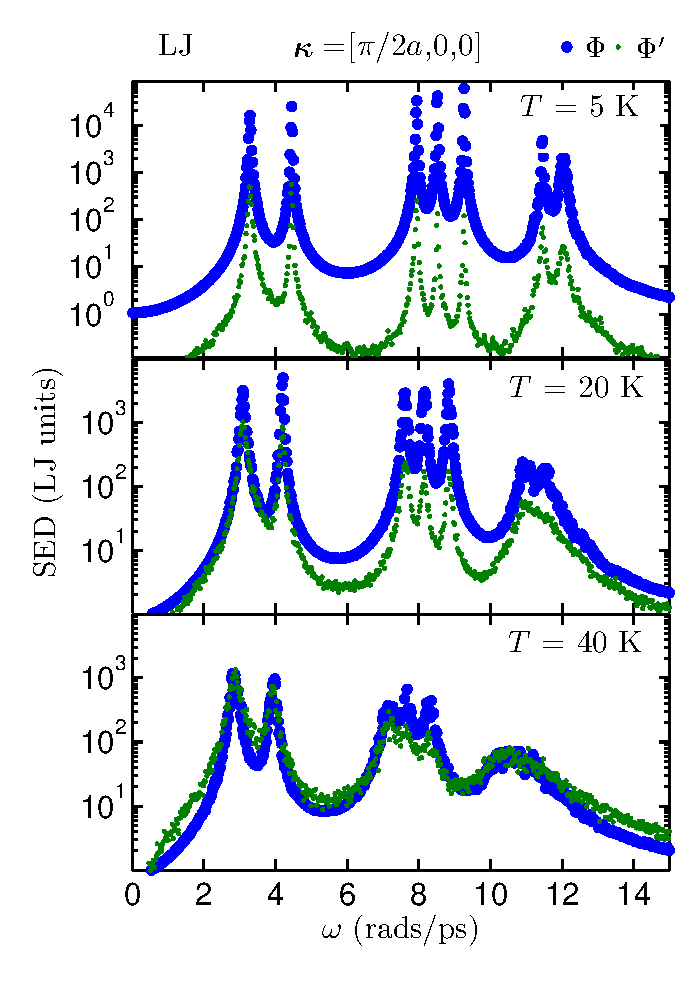
\includegraphics[angle=0,width=70.0mm]
{/home/jason/thesis/thesis/appendix/figure2.eps}
\vspace*{0mm}
\end{center}
\caption{\label{F:PEAK_COMPARE} The phonon spectral energy density 
($\Phi$) is plotted as 
larger blue circles.  The proposed alternative expression for the phonon 
spectral energy 
density ($\Phi'$) is plotted as smaller green points. The wavevector is 
($\pi/2a$,0,0). Note 
that peak broadening at higher temperatures and frequencies above $10$ 
rads/ps can force peaks 
close in frequency for $\Phi'$ to be fit as a single Lorentzian function. 
$\Phi$ does not suffer 
from this issue since the broadened peaks can be fit individually.}
\end{figure}
%--------------------------------------------------------------------------
\clearpage

The phonon frequencies and lifetimes extracted for all allowed wavevectors 
in the first Brillouin 
zone using $\Phi$ and $\Phi'$ at each of the three temperatures are 
compared on a mode-by-mode 
basis in Figs$.$ \ref{F:FREQ_LIFE_LJ}(a), \ref{F:FREQ_LIFE_LJ}(b), and 
\ref{F:FREQ_LIFE_LJ}(c). 
There, $\omega_0$, $\omega_0^{'}$, $\tau$, and $\tau^{'}$  refer to the 
mode properties predicted 
using $\Phi$ and $\Phi'$. The phonon frequencies agree well at all three 
temperatures, with 
increasing scatter at high temperatures and high frequencies.  This scatter 
is due to the high-frequency 
peak broadening seen in Fig$.$ \ref{F:PEAK_COMPARE} at $T = 40$ K, which 
can force peaks close in 
frequency for $\Phi'$ to be fit as a single Lorentzian function. The 
frequencies predicted by $\Phi$ 
and $\Phi'$ include the effects of anharmonicity, which increase the 
frequencies compared to the quasi-harmonic predictions 
\cite{mcgaughey_phonon_2006,turney_predicting_2009}. The agreement 
between the frequencies 
predicted from $\Phi$ and $\Phi'$ is explained in 
Appendix \ref{Appendix_B}.

The lifetimes show large scatter between $\Phi$ and $\Phi'$ on a 
mode-by-mode basis, with increasing 
scatter at high temperature that shows no systematic difference. The 
scatter at high frequencies 
is in part due to the peak broadening seen in Fig$.$ \ref{F:PEAK_COMPARE}, 
which can force peaks 
close in frequency for $\Phi'$ to be fit as a single Lorentzian function 
with a single lifetime. 
The broadening does not affect fitting at low frequencies, where the 
linewidths are much smaller 
than the peak spacings. There, any scatter comes solely from the difference 
between $\Phi$ and $\Phi'$.
%--------------------------------------------------------------------------
\begin{figure}
\begin{center}
\subfigure{
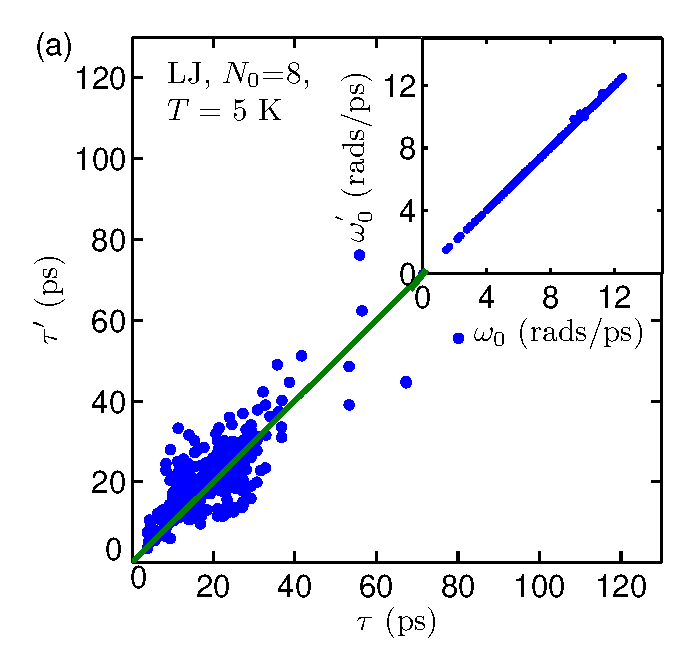
\includegraphics[angle=0,width=58.0mm]
{/home/jason/thesis/thesis/appendix/figure3_a.eps}
}
\subfigure{
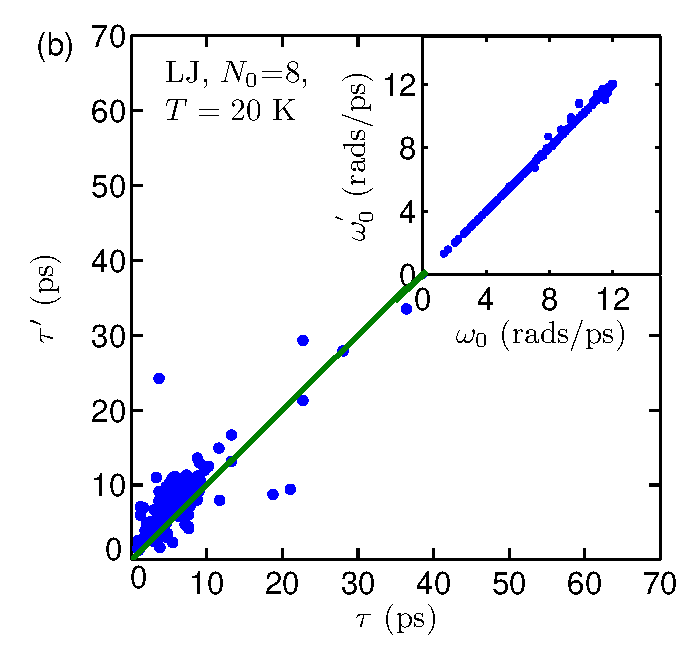
\includegraphics[angle=0,width=58.0mm]
{/home/jason/thesis/thesis/appendix/figure3_b.eps}
}
\subfigure{
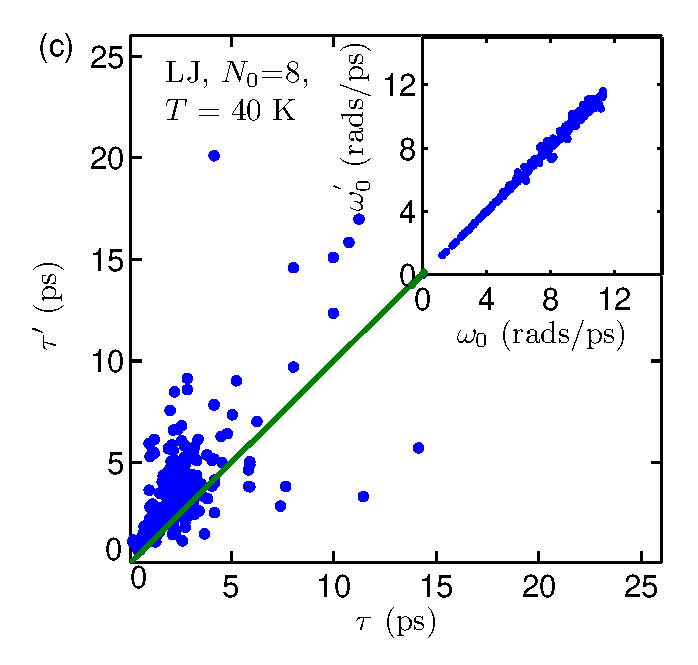
\includegraphics[angle=0,width=58.0mm]
{/home/jason/thesis/thesis/appendix/figure3_c.eps}
}
\end{center}
\caption{\label{F:FREQ_LIFE_LJ} Comparison of the phonon frequencies and 
lifetimes predicted using 
$\Phi$ ($\omega$ and $\tau$) and $\Phi'$ ($\omega^{'}$ and $\tau^{'}$) for 
LJ argon at temperatures 
of (a) 5 K, (b) 20 K, and (c) 40 K. The phonon frequencies agree well at 
all three temperatures, 
while the phonon lifetimes show large scatter.}
\end{figure}
%--------------------------------------------------------------------------
\clearpage

The phonon properties are then used to predict thermal conductivity using 
Equation 
\eqref{E-size:k_bulk}. The results are presented in Table 
\ref{T:cond_table}. The bulk thermal 
conductivities provided in Table \ref{T:cond_table} are predicted using 
the finite simulation-size 
scaling procedure discussed in \cite{turney_predicting_2009}. The bulk 
thermal conductivities predicted from 
$\Phi'$ are smaller and outside the uncertainty for those predicted from 
$\Phi$ for temperatures of 
$5$ and $20$ K. While the bulk thermal conductivities at a temperature of 
$40$ K agree within their 
uncertainties, the predicted mode-by-mode lifetimes show large scatter 
[Fig$.$ \ref{F:FREQ_LIFE_LJ}(c)] 
and the agreement should be regarded as coincidental.

The disagreement between $\Phi$ and $\Phi'$ in thermal conductivity comes 
directly from the differences 
in the phonon lifetimes. All other properties (frequencies, group 
velocities, specific heats) are 
nearly or exactly the same for the two calculations. The bulk thermal 
conductivities predicted from 
$\Phi$ and $\Phi'$ are also compared to predictions from the Green-Kubo 
method\cite{mcquarrie_statistical_2000} in 
Table \ref{T:cond_table}. For $N_1=N_2=N_3=8$, the thermal conductivity 
predicted by the Green-Kubo 
method is converged with respect to the simulation size 
\cite{mcgaughey_quantitative_2004}. The same MD data used 
to calculate $\Phi$ and $\Phi'$ is used for the Green-Kubo predictions. For 
all three temperatures, 
there is good agreement between the thermal conductivity predictions using 
$\Phi$ and Green-Kubo. For 
temperatures of $20$ and $40$ K, there is good agreement between the 
predictions from $\Phi$, Green-Kubo, 
and previous reports using non-equilibrium MD, anharmonic lattice dynamics, 
and time-domain $\Phi$ 
\cite{turney_predicting_2009}.
%--------------------------------------------------------------------------
\begin{center}
\begin{table}
\caption{\label{T:cond_table}Thermal conductivity values in W/m-K predicted 
using the $\Phi$, 
$\Phi'$, and Green-Kubo methods.  The predictions for $\Phi$ and Green-Kubo 
for the LJ system 
are in good agreement with those from other atomistic simulation methods
\cite{turney_predicting_2009} while 
those from $\Phi'$ differ and show no consistent behavior. The 
uncertainties in the predicted thermal 
conductivities for $\Phi$ and $\Phi'$ come predominantly from the finite 
simulation-size scaling 
procedure (see Ref. \cite{turney_predicting_2009,he_thermal_2011}), 
where the phonon 
properties and thermal conductivity 
are predicted for increasing system sizes ($N_1=N_2=N_3$) to extrapolate 
a bulk thermal conductivity. 
For SW silicon and the CNT, the extrapolation procedure is not performed. }
%\begin{ruledtabular}
\begin{tabular}{llllll}
     &                             &         &      &   \\
$T$ (K)&Green-Kubo \ &$\Phi$ &$\Phi'$\\
\hline
LJ (bulk)\\
5&8.0 $\pm$ 0.30 &7.9 $\pm$ 0.42 &5.8 $\pm$ 0.31 \\
20&1.3 $\pm$ 0.15 &1.2 $\pm$ 0.07 &1.0 $\pm$ 0.10 \\
40&0.45 $\pm$ 0.07 &0.47 $\pm$ 0.03 &0.49 $\pm$ 0.05 \\
\hline
SW ($N_1=N_2=N_3=6$) \\
300& &322 $\pm$ 16 &396 $\pm$ 38 \\
\hline
CNT ($N_1=N_2=1, N_3=50$) \\
300& &428 $\pm$ 21 &398 $\pm$ 40 \\
\end{tabular}
%\end{ruledtabular}
\end{table}
\end{center}
%--------------------------------------------------------------------------
\clearpage

%--------------------------------------------------------------------------
\subsection{\label{S:Subsection_prop_SW}Stillinger-Weber Silicon}
%--------------------------------------------------------------------------
We next compare the phonon properties and thermal conductivity predicted 
from $\Phi$ and $\Phi'$ 
for SW silicon \cite{stillinger_computer_1985} at a temperature of 
$300$ K and zero pressure with a lattice 
constant of 5.437 $\AA$. The SW system is stiffer (larger phonon group 
velocities, frequencies, and 
lifetimes) than LJ argon and is an additional test to determine if there 
is a systematic error in 
the predictions from $\Phi'$. The MD simulations are performed using 
LAMMPS \cite{plimpton_fast_1995}. The MD 
system consists
of $N_1 \times N_2 \times N_3 = 6^3 = 216$ conventional unit cells for a 
total of 1728 atoms 
($b=8$ atoms). The phonon frequencies, eigenvectors, and group velocities 
are generated using 
GULP \cite{gale_general_2003}.

Using a 0.5 fs timestep, the system is equilibrated for $2^{20}$ time 
steps before collecting 
data every $2^5$ time step for $2^{22}$ time steps in the $NVE$ ensemble 
\cite{mcquarrie_statistical_2000}. 
As with the LJ system, the sampling rate is determined by the highest 
phonon frequency in the 
system. Five simulations with different initial conditions are performed 
and the $\Phi$ and $\Phi'$ 
values are averaged before the peak fitting. $\Phi$ and $\Phi'$ are 
further averaged over degenerate 
wavevectors in the Brillouin zone, reducing the wavevectors to the first 
octant \cite{mcgaughey_phonon_2004}.

The extracted phonon frequencies and lifetimes are plotted in Fig$.$ 
\ref{F:FREQ_LIFE_Si}. 
As with the LJ system, the phonon frequencies are predicted accurately 
by $\Phi'$ but the 
lifetimes show large scatter on a mode-by-mode basis. For the system 
size studied, $\Phi'$ 
predicts a larger thermal conductivity than $\Phi$ outside the prediction 
uncertainties, in 
contrast to the LJ system (see Table \ref{T:cond_table}). The disagreement 
in thermal conductivity comes directly from the phonon lifetimes.

\vspace*{1mm}
%--------------------------------------------------------------------------
\begin{figure}
\begin{center}
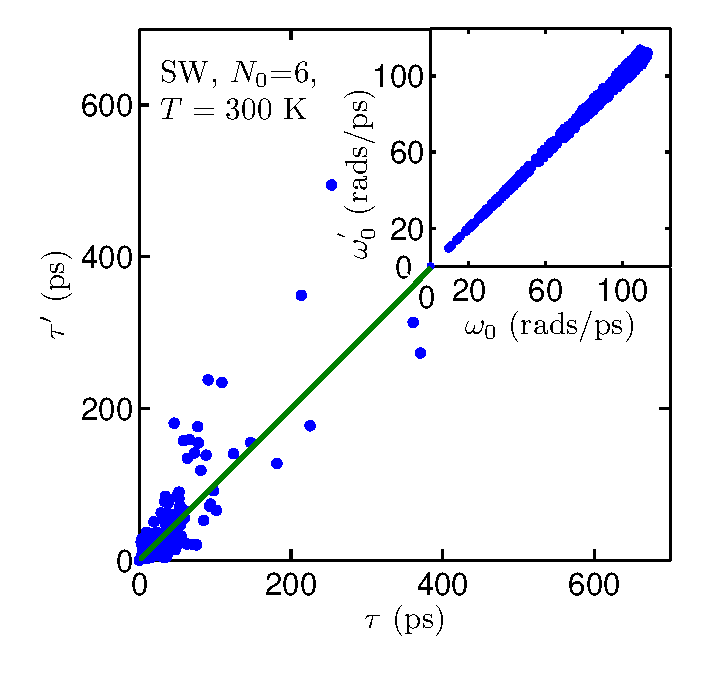
\includegraphics[angle=0,width=70.0mm]
{/home/jason/thesis/thesis/appendix/figure4.eps}
\vspace*{0mm}
\end{center}
\caption{\label{F:FREQ_LIFE_Si} Comparison of the phonon frequencies and 
lifetimes predicted 
using $\Phi$ ($\omega$ and $\tau$) and  $\Phi'$ ($\omega'$ and $\tau'$) 
for SW silicon. The 
phonon frequencies agree well, while the phonon lifetimes show large 
scatter.}
\end{figure}
%--------------------------------------------------------------------------
\clearpage

%--------------------------------------------------------------------------
\subsection{\label{S:Subsection_prop_CNT}Carbon Nanotube}
%--------------------------------------------------------------------------
Finally, we compare the phonon properties and thermal conductivities 
predicted by $\Phi$ and 
$\Phi'$ for an (8,8) CNT (diameter of 1.10-nm and length of 12.3 nm) at 
a temperature of $300$ K 
and zero pressure \cite{thomas_predicting_2010}. 
The interactions in the CNT system 
are modeled using the 
REBO potential without the four-body interaction term 
\cite{brenner_second-generation_2002}. 
The MD simulations are 
performed using an in-house code. The MD system consists of 1600 atoms 
(32 atoms/unit cell). The 
phonon frequencies, eigenvectors, and group velocities are generated using 
an in-house code. The 
purpose of simulating this system is to check the results of Thomas et al.
\cite{thomas_predicting_2010} (who 
used $\Phi'$ and non-equilibrium MD), and to compare the predictions of 
$\Phi'$ and $\Phi$.

Using a 1.0 fs timestep, the system is equilibrated for $2^{20}$ time 
steps before collecting data 
every $2^3$ time step for $2^{22}$ time steps in the $NVE$ ensemble 
\cite{mcquarrie_statistical_2000}. As with 
the LJ and SW systems, the sampling rate is determined by the highest 
phonon frequency in the 
system. Five simulations with different initial conditions are performed 
and the $\Phi$ and $\Phi'$ 
values are averaged before the peak fitting. Since the Brillouin zone of 
the CNT is 
one-dimensional, $\Phi$ and $\Phi'$ are further averaged over 
directionally-degenerate wavevectors.

The phonon frequencies and lifetimes for the allowed wavevectors in the 
one-dimensional Brillouin 
zone are shown in Fig. \ref{F:FREQ_LIFE_CNT}. Like the LJ and SW silicon 
systems, the 
phonon frequencies can be predicted accurately by $\Phi'$, but the 
lifetimes show large scatter. 
The estimated thermal conductivity of the CNT predicted using $\Phi'$ is 
in agreement with the 
results of Thomas et al. \cite{thomas_predicting_2010}. 
The thermal conductivity 
predicted by $\Phi'$ is less 
than that predicted by $\Phi$, but not outside their uncertainties.

\vspace*{1mm}
%--------------------------------------------------------------------------
\begin{figure}
\begin{center}
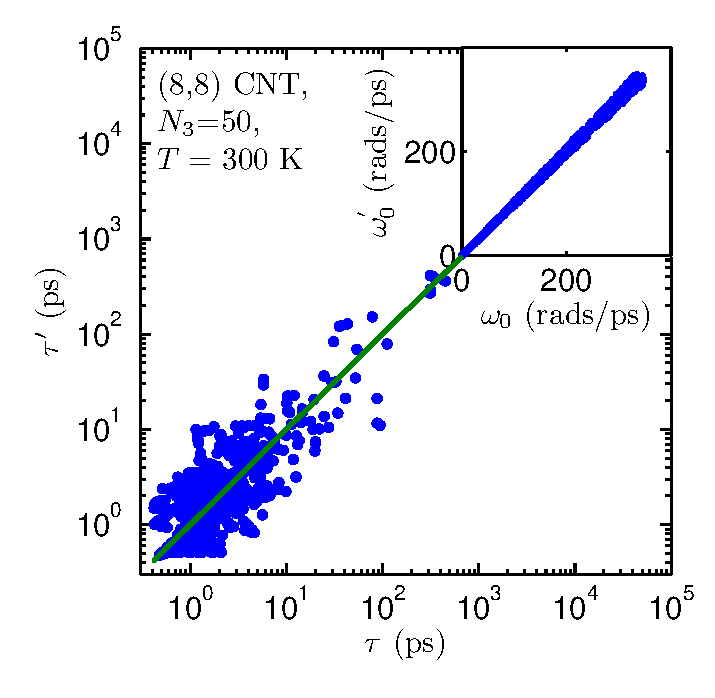
\includegraphics[angle=0,width=70.0mm]
{/home/jason/thesis/thesis/appendix/figure5.eps}
\vspace*{0mm}
\end{center}
\caption{\label{F:FREQ_LIFE_CNT} Comparison of the phonon frequencies and 
lifetimes predicted 
using $\Phi$ ($\omega,\tau$) and $\Phi'$ ($\omega',\tau'$) for a (8,8) CNT 
modeled using the REBO 
potential. The phonon frequencies agree well, while the phonon lifetimes 
show large scatter.}
\end{figure}
%--------------------------------------------------------------------------
\clearpage

%--------------------------------------------------------------------------
\section{\label{Section_Conclusions}Summary}
%--------------------------------------------------------------------------
We presented the correct phonon SED, $\Phi$, and its relation to the phonon 
frequencies and lifetimes. 
We then presented an alternative formulation to the 
phonon spectral energy density, $\Phi'$, which does not require the phonon 
mode eigenvectors.  
Because $\Phi'$ does not contain the eigenvectors, this alternative 
formulation does not represent 
the phonon spectral energy density, but does contain information about 
the phonon dispersion as the 
temperature approaches $0$ K (see Appendix \ref{Appendix_B}).

We then calculated the phonon SED for LJ argon, SW silicon, and a CNT 
modeled with the REBO 
potential using $\Phi$ and $\Phi'$. The phonon frequencies and
lifetimes predicted from $\Phi$ and $\Phi'$ are shown in Figs$.$ 
\ref{F:FREQ_LIFE_LJ}, 
\ref{F:FREQ_LIFE_Si} and \ref{F:FREQ_LIFE_CNT}. The
frequencies are in good agreement between the two SED methods, while the 
lifetimes show large scatter.

The phonon SED $\Phi$ is well-defined theoretically, while $\Phi'$ does 
not properly map to the 
phonon energies since it is missing the phonon mode eigenvector. We deduce 
that this is the reason 
$\Phi'$ does not accurately predict the phonon lifetimes. It is surprising 
how close the predicted 
thermal conductivities can be using $\Phi$ and $\Phi'$ (LJ at $T=40$ K and 
the CNT results). The 
thermal conductivities predicted by $\Phi$ and $\Phi'$, however, show no 
consistency for the three 
systems studied.

The most important predictions are the mode-by-mode phonon properties. Of 
particular importance are 
the lifetimes, which are the key input for Boltzmann transport 
equation-based models 
\cite{mcgaughey_size-dependent_2011}. Thus, we do not recommend $\Phi'$ 
for predicting phonon lifetimes or 
thermal conductivity.  Any agreement in thermal conductivity predictions 
between atomistic 
studies\cite{thomas_predicting_2010} and experiment
\cite{koker_thermal_2009,qiu_molecular_2011} should 
be regarded as 
coincidental, and the phonon lifetime reductions predicted for systems 
with additional scattering 
methods \cite{thomas_predicting_2010,shiomi_thermal_2011} should only 
be interpreted qualitatively. The use of $\Phi'$ 
in future work is discouraged and we reccomend the use of $\Phi$.


% \ack
% This work is supported by AFOSR award FA95501010098. We thank John A. 
% Thomas (Johns Hopkins 
% University Applied Physics Laboratory) for helpful discussions.
% %\end{acknowledgments}

